\documentclass[12pt,norsk,a4paper]{article}
\usepackage[norsk]{babel}
\usepackage[norsk]{isodate}
\usepackage[T1]{fontenc}
\usepackage{parskip}
\usepackage{url}
\usepackage{listings}
\usepackage{gensymb}
\author{fridatbe}
\title{IN1080 --- Obligatorisk oppgave 3}
\date{\today}
\usepackage[small,euler-digits]{eulervm}
\usepackage{color}
% \usepackage{minted}
\usepackage{xcolor}
\definecolor{LightGray}{gray}{0.9}
\usepackage{a4wide}
\usepackage[top=2cm]{geometry}
\usepackage{graphicx}
\graphicspath{ {./fig/} }
\newcommand{\tuple}[1]{\ensuremath{\langle #1\rangle}}
\newcommand{\set}[1]{\ensuremath{\{#1\}}}
\newcommand{\imp}{\ensuremath{\rightarrow}}
\newcommand{\M}{\ensuremath{\mathcal{M}}}
\newcommand{\AF}{edge from parent[draw=none]}
\newcommand{\NODE}[1]{\{node \{\ensuremath{#1}\}\}}
\usepackage[explicit]{titlesec}
\titleformat{\section}{\normalfont\Large\bfseries}{}{0em}{#1\ \thesection}


\begin{document}
    \maketitle
    \renewcommand{\thesubsection}{(\alph{subsection})}
    \newpage

    \section{Oppgave}
        Figur:\\
        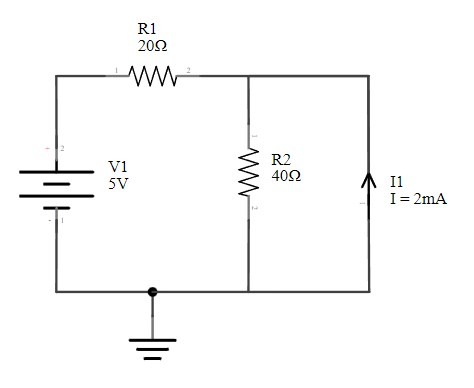
\includegraphics[width=0.5\textwidth]{opg1.jpg}\\
        Kirchoff's strømlov: summen av strømmene inn og ut av en node er lik 0\\
        Finn strømmen gjennom R2:\\
        Tar utgangspunkt i noden der strømmen  gjennom $R_1, R_2$ og $I1$ møtes\\
        $I_{R1} + (- I_{R2}) + I1 = 0$\\
        $I_{R2} = I_{R1} + I1$\\\\
        Finner strømmen gjennom R2 fra venstre (fjerner strømkilden og ser på kretsen som seriell):\\
        $I_{venstre} = \frac{V1}{R1+R2} = \frac{5V}{20 Ohm + 40 Ohm} = 0.083A = 83mA$\\\\
        Finner strømmen gjennom R2 fra høyre (kortslutter V1 og ser på kretsen som parallell):\\
        $I_{høyre} = I1\frac{(R1||R2)}{R2}$\\\\
        $R1||R2 = \frac{R1*R2}{R1+R2} = \frac{20 Ohm * 40 Ohm}{20 Ohm + 40 Ohm} = 13.3 Ohm$\\\\
        $I_{høyre} = 2mA *\frac{13.3 Ohm}{40 Ohm} = 0.67mA$\\\\\\
        Den totale strømmen gjennom R2 blir da:\\\\
        \underline{$I_{R2} = I_{høyre} + I_{venstre} = 0.67mA + 83mA = 83.67mA$}

        % Siden R1 er koblet i serie med kilden og strømmen ikke går gjennom noen andre strømdelere før den, vil $I_{R1} = I_{tot}$\\
        % Finner da $I_{R1}$:
        % $I_{R1} = V1/R1$\\
        % $I_{R1} = 5V / 20 Ohm = 0.25A$\\\\
        % Setter svaret inn i formel (Kirchoff's strømlov), og har allerde oppgitt I1 = 2mA\\
        % $I_{R2} = 0.25A - 2mA$\\
        % $I_{R2} = 0.25A - 0.002A$\\
        % \underline{$I_{R2} = 0.248$}

        % $V_{x} = V1 * \frac{R2}{R1+R2}$
        % $V_{x} = 5V * \frac{40 Ohm}{20 Ohm + 40 Ohm}$
        % $V_{x} = 3.33V$

        % $I_{x} = \frac{3.33V}{40 Ohm}$
        % $I_{x} = 0.083A = 83mA$
        % Bruker Kircchoffs strømlov gir:
        % $I_{R2} = 83mA - 2mA = 81mA$
        % $I_{R2} = 0.081A$

    \newpage

    \section{Oppgave}
        Figur:\\
        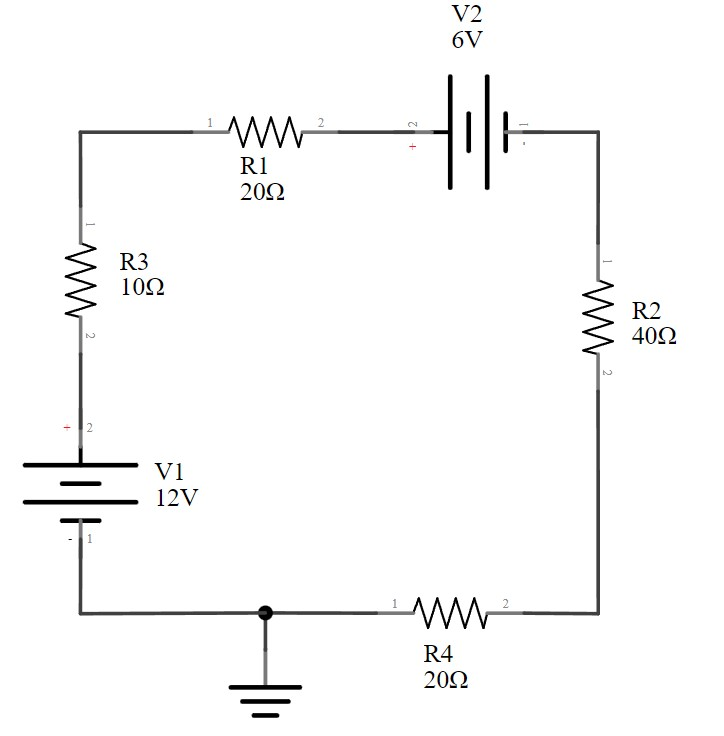
\includegraphics[width=0.5\textwidth]{opg2.jpg}\\

        Kirchoffs spenningslov gir:\\\\
        $V1 + V2 = V_{R1} + V_{R3} + V_{R2} + V_{R4}$\\\\
        $V1 + V2 = (I_{R1}*R1) + (I_{R3}*R3) + (I_{R2}*R2) + (I_{R4}*R4)$\\\\
        Siden kretsen er seriell, er strømmen lik gjennom hele kretsen (V2 har negativt fortegn på grunn av motsatt polaritet av V1):\\
        $V1 - V2 = I*(R1+R2+R3+R4)$\\\\
        $I = \frac{V1-V2}{R1+R2+R3+R4} = \frac{12V - 6V}{20 Ohm + 40 Ohm + 10 Ohm + 20 Ohm} = \frac{6 V}{90 Ohm}$\\\\
        $I = 0.0667 A$\\\\
        Finner da spenning over R2:\\\\
        $V_{R2} = R2 * I = 40 Ohm * 0.0667$\\\\
        \underline{$V_{R2} = 2.67 V$}\\\\
        Sjekker svaret med Kirchoffs spenningslov:\\
        $12V - 6V = 2.67 + 0.0667A*(20 Ohm + 10 Ohm + 20 Ohm) = 6.005V$\\\\

        % Formel for superposisjon gir også samme verdi:\\\\
        % $V_{R2} = V_{tot source} * \frac{R2}{R1 + R2 + R3 + R4} = (12V - 6V) * \frac{40 Ohm}{20 Ohm + 40 Ohm + 10 Ohm + 20 Ohm} = 6V * \frac{40 Ohm}{90 Ohm}$\\\\
        % \underline{$V_{R2} = 2.67V$}\\\\



    \newpage

    \section{Oppgave}
        Figur:\\
        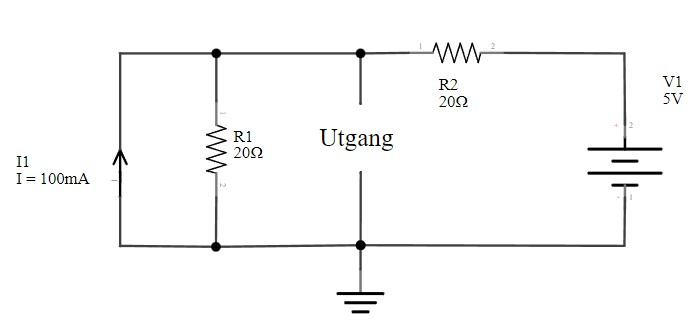
\includegraphics[width=1\textwidth]{opg3.jpg}\\
        % Bruker superposisjon for å kortslutte og se på en og en krestdel
        Spenning over utgangen:\\
        Ser på kretsen som en Thevenin krets:\\
        $V_{utgang} = V1/n$ (n er antall like resistorer)\\
        $V_{utgang} = 5V/2 = 2.5V$\\\\
        Ser på kretsen som en Norton krets:\\
        $V = I * R$\\
        $V = 100mA * \frac{20 Ohm * 20 Ohm}{20 Ohm + 20 Ohm} = 0.1A * \frac{20 Ohm * 20 Ohm}{20 Ohm + 20 Ohm} = 0.1A * \frac{400 Ohm}{40 Ohm}$\\
        $V = 1V$\\\\
        Total spenning over utgang:\\
        \underline{$V_{tot} = 1V + 2.5V = 3.5V$}\\\\
        Resistans (resistorene ligger i parallell):\\
        $R_{tot} = \frac{R1*R2}{R1+R2} = \frac{20 Ohm * 20 Ohm}{20 Ohm + 20 Ohm} = \frac{400 Ohm}{40 Ohm}$\\
        \underline{$R_{tot} = 10 Ohm$}\\

    \newpage

    
    \section{Oppgave}
    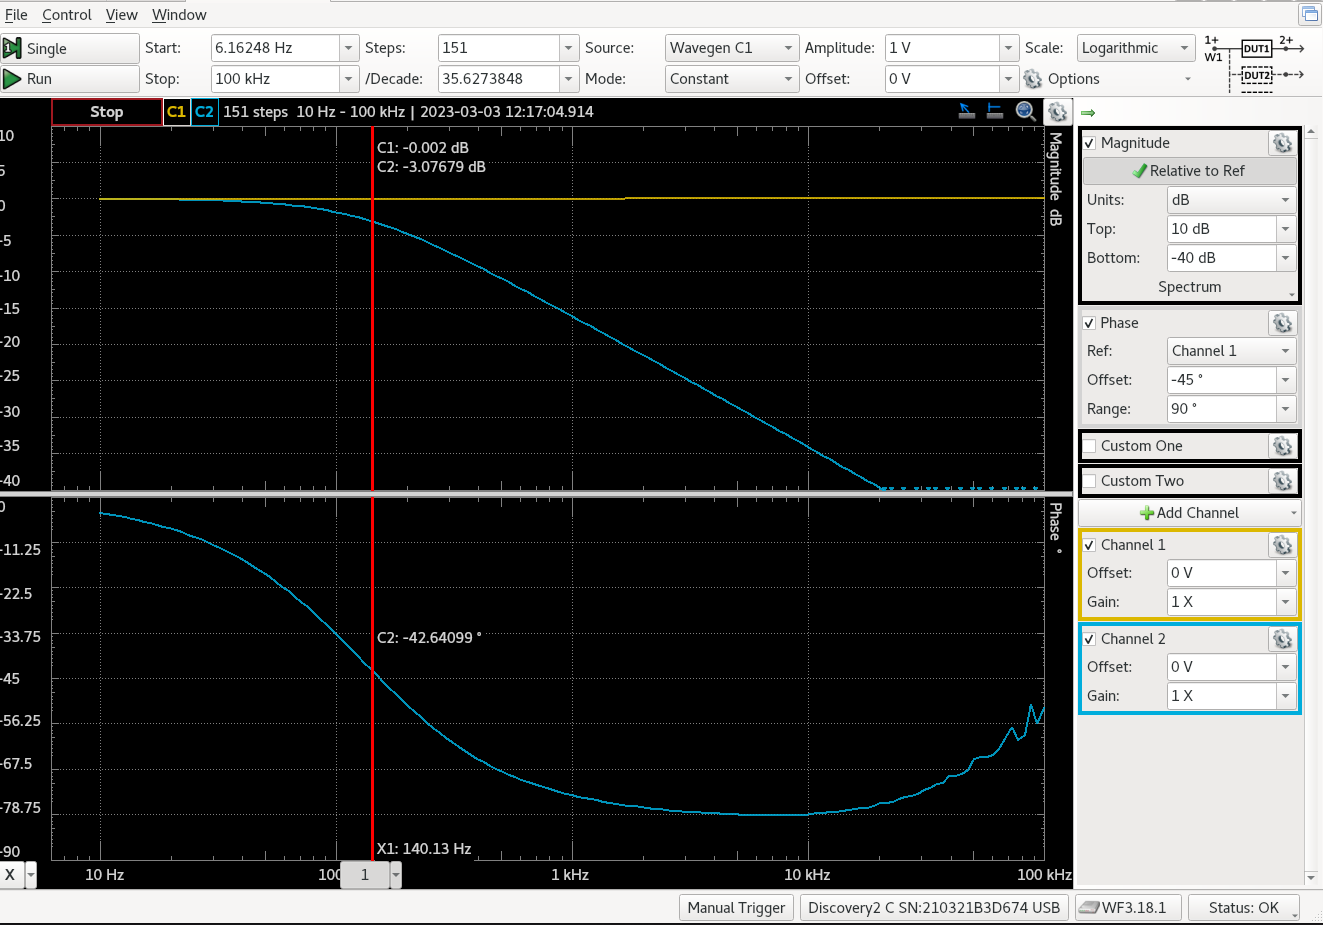
\includegraphics[width=1\textwidth]{screen.png}\\\\
    Teoretiske beregninger:\\
    Grensefrekvensen (ved -3dB): $f = \frac{1}{2*\pi*R*C} = \frac{1}{2*\pi*1KOhm*1uF} = \frac{1}{2*\pi*1000Ohm*0.000001F} = 159.15Hz$\\
    Fasen (ved -3dB): $arcsin(\frac{1}{\sqrt{2}})= \frac{\pi}{4} = 45^{\circ}$\\\\\\

    Praktiske målinger:\\
    Grensefrekvensen (ved -3dB): X1 = 140.13Hz\\
    Fasen (ved -3dB): $X2 = 42.64^{\circ}$\\\\\\

    I praksis er både fasen og grensefrakevensen noe lavere. Dette kan blandt annet være fordi markøren ikke er helt nøyaktig på -3.0dB.
    \newpage



\end{document}
